\documentclass[12pt]{article}
\usepackage[utf8]{inputenc}
\usepackage{amsmath}
\usepackage{amsfonts}
\usepackage{amssymb}
\usepackage{enumitem}


% this is to make it look like a word document.
\usepackage[tmargin=0.98in,bmargin=0.98in,lmargin=1.18in,rmargin=1.18in]{geometry}

% package necessary to add pictures to latex
\usepackage{graphicx}

\title{\vspace{-4ex}RoboCup@Work:\\Compitiendo por la fábrica del futuro\vspace{-2ex}}
\date{\today}
\author{Luis Servín\\ Taller TRA, Universidad Nacional Autónoma de México}

\begin{document}

\maketitle

\section*{Resumen}

RoboCup@Work se enfoca en el uso de manipuladores manipuladores móviles y su integración con equipo de automatización para el desarrollo de tareas relevantes dentro de la industria.

\section{Introducción}

Recientemente, tanto la robótica como la automatización industrial están cambiando su campo de atención hacia escenarios en los cuales se ve envuelta la integración de distintos factores como: movilidad y manipulación, integración a gran escala de robots tanto de servicio como industriales, espacios cohabitados entre humanos y robots, así como la colaboración entre múltiples robots y humanos. Todas estas ideas se pueden considerar parte de \emph{la fábrica del futuro} ó FoF por sus siglas en ingles \cite{tapas2013}.

Un componente esencial de la FoF son los \textbf{manipuladores móviles} los cuales son una combinan las cualidades de un robot móvil con las capacidades de uno o más manipuladores. Este campo ha llevado al desarrollo de distintas plataformas de investigación. Algunos ejemplos son youBot \cite{bischoff2011kuka} y omniRob por parte de KUKA y rob@worlk por  Fraunhofer IPA.

\section{Temas de Investigación y Retos}

La competencia RoboCup@Work tiene como objetivo el uso de robots en ambientes de trabajo y aborda retos de investigación aun abiertos en robótica industrial y de servicio. Algunos ejemplos de los posibles escenarios son:

\begin{itemize}[noitemsep]
	\item Carga y descarga de objetos de distintos tamaño.
	\item Recoger y entregar objetos desde y hacia almacenes no necesariamente estructurados.
	\item Operación de maquinaria, presionar botones, abrir y cerrar puertas, algunas otras operaciones que no tengan una cinemática definida.
	\item Planeación flexible y programación dinámica de distintos procesos.
	\item Ensamble cooperativo de objetos no triviales entre robots y/o humanos.
	\item Recolección cooperativa de objetos a gran escala en ambientes amplios.
	\item Transportación cooperativa de grandes objetos c/s humanos.
\end{itemize}

\section{Diseño de la Competencia}

\subsection{Visión e Ideas Generales}

Ser atractivo para el público es uno de los objetivos primordiales. Se busca el uso de robot pequeños en lugar de grandes manipuladores industriales, para con ello mantener el área de competencia pequeña.

Al respecto de la estructura se buscan como elementos básicos tener pruebas bien definidas, que se enfoquen en la realización de tareas específicas.

Para la puntuación, se definieron objetivos claros y criterios de desempeño claros para cada de las pruebas y tareas a desarrollarse por el robot. Premios son dados debido a logros específicos o un desempeño destacable en alguna tarea o funcionalidad que sea requerida. (\emph{best-in-class})

\subsection{Arena de Competencia RoboCup@Work}

El escenario fue inicialmente diseñado para la competencia como el que se muestra en la figura \ref{fig:arena_concept}. Este diseño se trata solamente de un primer ejemplo, ya que dicho ambiente debe poderse adaptar dentro de ciertos márgenes razonables.

\begin{figure} [h!]
	\centering
	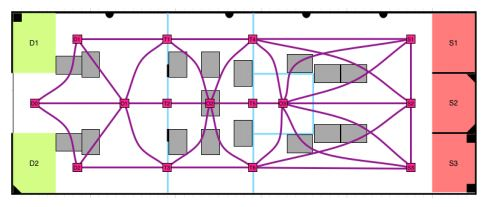
\includegraphics[scale=1]{images/arena_first_concept.JPG}
	\caption{Concepto de arena de competencia}
	\label{fig:arena_concept}
\end{figure}

\subsection{Objetos para Manipulación y Cavidades Utilizadas}

Los objetos a manipular utilizados dentro de la competencia deber tener una aplicación relevante dentro de la industria. Además se tiene que tratar de elementos estandarizados bajos las normativas DIN o ISO, y estar disponibles ámpliamente alrededor del mundo. Estos presentan retos demandantes en términos de detección (i.e. tornillos relativamente pequeños) y reconocimiento (i.e. hacer distinción entre tuercas que difieren solamente por la estructura de su superficie.

\subsection{Prueba Básica de Navegación (BNT: Basic Navigation Test)}

Tiene como objetivo que los equipos demuestren su habilidad para navegar de manera segura en el área de competencia, i.e. teniendo un objetivo claro y específico, autónomamente, robusto, y de manera segura.

\subsection{Prueba Básica de Manipulación (BMT: Basic Manipulation Test)}

Se trata de la segunda prueba, en la cual los equipos deben demostrar su habilidad para percibir objetos y realizar operaciones de pick and place con ellos. Su foco de atención se centra en la manipulación, además de demostrar que se pueden desarrollar tareas de pick and place de manera segura y robusta con objetos de distintas formas y tamaños.

\subsection{Prueba Básica de Transporte (BTT: Basic Transportation Test)}

Como parte de la tercera prueba, los equipos deben demostrar su habilidad para navegar y manipular objetos al desarrollar tareas simples de transportación.

\section{Implementación: Primeros pasos de la liga}

\emph{Construyendo una comunidad}: La idea inicial de la competencia fue inicialmente desarrollado bajo el proyecto BRICS. El cual tiene como objetivo principal estructurar y formalizar el proceso de desarrollo de sistemas robóticos, además de proveer de proveer de herramientas, modelos y bibliotecas de software, las cuales ayuden a acelerarlo \cite{brics2015}.

En mayo de 2012, se organizó el primer campamento RoboCup@Work en la universidad de Bonn-Rhein-Sieg (BRSU).

\emph{Desarrollo de la infraestructura}: Un grupo de trabajo en la BRSU diseñó y construyó una nueva arena para la competencia de 2013, con base en perfiles de aluminio de alta calidad.

Uno de los mayores retos se presentó al momento de seleccionar el conjunto de elementos a utilizar durante las pruebas de manipulación. Estos debían ser objetos industriales reales, suficientemente grandes para ser percibidos por las tecnologías actuales, además de suficientemente ligeros y pequeños para ser sujetados y manipulados por la plataformas de investigación propuestas.

Se diseño además una plataforma que permite definir las especificaciones para cada tarea y transmitirlas a los robots. Además debería ser capaz de mantener un registro del tiempo y mandar señales de inicio y fin. La primera versión de esta plataforma \emph{refere box} fue desarrollada dentro de la BRSU.

\bibliographystyle{ieeetran}
\bibliography{bibliography}

\end{document}
























